This distribution is again similar to the mixed distribution.
With probability 1/2 the value is chosen from the overlapped distribution and with remaining probability 1/2 the value is chosen from the mixed distribution.

\begin{figure}[h]
      \caption{Distribution of a mixed and overlapped input with \textasciitilde$U(1,999)$, \textasciitilde$B(1000.0.1)$, \textasciitilde$Geo(0.01)$, powerlaw dist with $\beta=-1.25$}
      \centering
      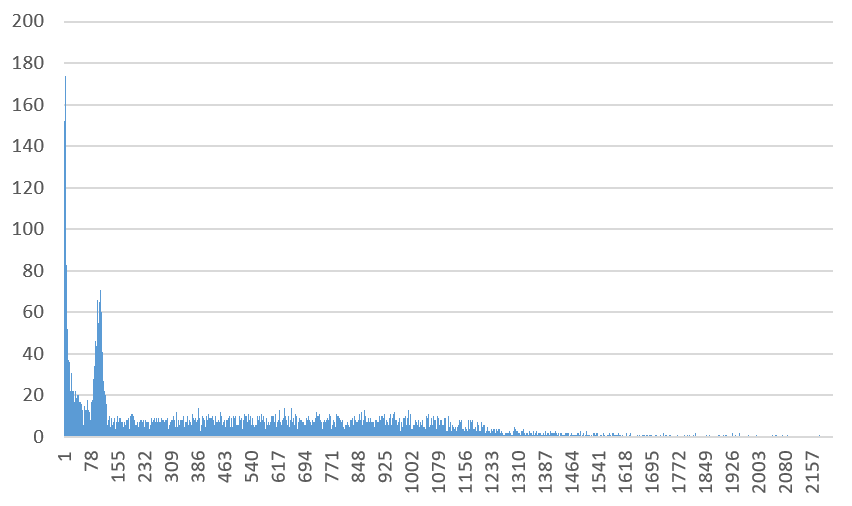
\includegraphics[width=0.7\textwidth]{figures/images/numberGenerator/mixedAndOverlapped.png}\label{fig:mixAndOverlDistExample}
\end{figure}

The used distributions were \textasciitilde$U(1,49999)$, \textasciitilde$B(10000.0.1)$, \textasciitilde$Geo(0.001)$, powerlaw dist with $\beta=-1.25$.
By looking at Figure~\ref{fig:mixAndOverlDistExample} it looks like the mixed and overlapped distribution is closer to the mixed distribution than to the overlapped distribution.
The results should also be closer to the mixed distribution.